\chapter{Calibrated Latent Models for Value Aware Model Learning}
\label{chap:cvaml}

\begin{quote}
    This chapter is based on \longfullcite{voelcker2025calibrated} and \longfullcite{voelcker2023lambda}.
\end{quote}

\newcommand{\rev}[1]{#1}

\section{Introduction}
In model-based reinforcement learning, an agent collects information in an environment and uses it to learn a model of the world. 
This model is used to improve value estimation and policy learning~\parencite{dyna,deisenroth2011pilco, hafner2020dream,schrittwieser2020mastering}.
However, as environment complexity increases, learning a model becomes more and more challenging. 
This leads to model errors which propagate to value function learning~\parencite{schneider1997exploiting,kearns2002near,talvitie2017self,lambert202objective}.
In such cases, deciding what aspects of the environment to model is crucial.

The paradigm of \emph{value-aware model learning} (VAML)~\parencite{vaml} and \emph{value-equivalence}~\parencite{grimm2020value,grimm2021proper} addresses this by training models that lead to accurate value estimation.
Prominent value-aware model learning approaches are MuZero~\parencite{schrittwieser2020mastering} and IterVAML~\parencite{itervaml}.
The MuZero loss has been shown to perform well in discrete~\parencite{schrittwieser2020mastering,ye2021mastering} and continuous control tasks~\parencite{hansen2022temporal,hansen2024tdmpc}, but has received little theoretical investigation.
On the other hand, IterVAML is a theoretically motivated algorithm but not commonly used in empirical work.
We show that MuZero and IterVAML can be unified in a family of losses, which we term $(m,b)$-Value-Aware Model Losses ($(m,b)$-VAML).
The name stresses the two core hyperparameters: the model rollout steps, $m$, and steps used to estimate the bootstrapped value function target, $b$.

The $(m,b)$-VAML losses are used as surrogate losses in place of other value- or model learning losses.
Therefore, it is important to ask whether they are calibrated \parencite{steinwart2008support}.
A calibrated loss does not lead to suboptimal minima when the function class includes optimal functions for the original target loss.

\textbf{Research question:} This chapter has three parts, each with a theoretical and empirical section. We answer two questions about the $(m,b)$-VAML family: (a) What variants of the $(m,b)$-VAML losses are well-calibrated to recover correct models and value functions? (b) How do deterministic latent-model architectures impact the stability of $(m,b)$-VAML algorithms? (c) Do we observe problems with uncalibrated losses when using stochastic architectures?

\textbf{Contributions:} 
As our main theoretical contribution, we mathematically analyze the family of $(m,b)$-VAML algorithms.
We prove that all members of this loss family are uncalibrated when used with a stochastic environment model.
To counter this issue, we derive a novel loss variant.

In the second part, we address issues arising from the way current algorithms in the $(m,b)$-VAML family are commonly implemented.
We prove that a stochastic model class is not necessary to learn a single-step decision-equivalent model in stochastic environments.
This validates the practice of primarily using deterministic models in empirical work~\parencite{oh2017value,schrittwieser2020mastering,hansen2022temporal}.
Empirically we find that using stochastic models can still lead to improved performance, although this is environment-dependent.


\section{Notation}

\textbf{Reinforcement Learning:} We consider a standard as presented in \autoref{chap:background:mdp}.
As a brief reminder, we review the notation.
The policy-conditioned transition kernel is $\P^\pi(x'|x) = \int \P(x'|x,a) \pi(a|x) \mathrm{d} a.$
The value is the unique stationary point of the Bellman operator $$[\mathcal{T}_{\P^\pi} V](x) = \EEX{\pi}{r(x_0,a_0) + \gamma  \EEX{\P^\pi}{V(x_1)}|x_0=x}.$$
This operator can be extended to a multi-step version as $$[{\mathcal{T}}^b_{\P^\pi} V](x) = \EEX{\pi,\P}{\sum_{n=0}^{b-1} \gamma^n r(x_n,a_n) + \gamma^b {V(x_b)}\Big|x_0=x}.$$
We also define $[\mathcal{T}_{\P^\pi}^0 V](x) = V(x).$

\textbf{Model-based RL:} In this chapter, we focus on value learning with model data, which is commonly referred to as Dyna~\parencite{dyna}.
We use $\hat{p}$ to refer to a stochastic model, and $\hat{f}$ for deterministic models.
When a model is used to predict the observation $x'$ from $x,a$ (such as the model used in \ac{mbpo} \parencite{janner2019mbpo}) we call it an \emph{observation-space models}.
Alternatively, \emph{latent-space models} of the form $\hat{p}(z'|z, a)$ are used, where $z\in\mathcal{Z}$ is a representation of a state $x\in\mathcal{X}$ given by $\phi: \mathcal{X} \rightarrow \mathcal{Z}$.
Observation-space models predict next states in the representation of the environment, while latent-space models reconstruct learned features of these states.

The notation $x^{(n)}$ refers to the $n$-th step in a rollout starting in state $x$ in the environment.
We will use $\hat{x}^{(n)}$ to refer to samples from the $n$-th step model prediction and write $\EEX{\hat{p}}{\cdot}$ as a shorthand for $\EEX{{x}^{(m)}\sim \hat{p}(\cdot|x)}{\cdot}$.

\section{The Value-Aware Model Learning framework}
\label{sec:cvaml:model_losses}

\begin{figure*}[t]
    \centering
    \begin{minipage}{0.63\linewidth}
        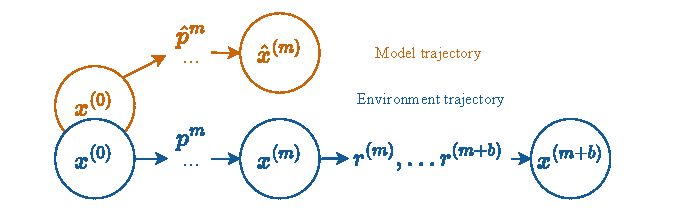
\includegraphics[width=\linewidth]{figures/lambda/mb_loss.drawio.pdf}
    \end{minipage}
    \begin{minipage}{0.36\linewidth}
    \begin{align}
        &\hat{\mathcal{L}}^{\P^\pi}_{m,b}\left(\hat{p},\hat{V}|x\right)\\
        = &\biggl|{\color{newgreendeal}\underbrace{\hat{V}\roundb{\hat{x}}}_\mathrm{model}} - 
        \biggl[ {\color{newbluedeal} \underbrace{[\mathcal{T}_{\P^\pi}^b \hat{V}]\roundb{x^{(m)}} }_\mathrm{environment} } \biggr]_\mathrm{sg}\biggr|^2
    \end{align}
    \end{minipage}
    \caption{Sketch of $(m,b)$-VAML. The loss is computed from an {\color{newgreendeal}$m$-step model} and a {\color{newbluedeal} $(m+b)$-step environment trajectory}. It is the difference between the estimated value of the {\color{newgreendeal}$m$-th model state}, and the $b$-step Bellman operator starting from the {\color{newbluedeal} $m$-th environment state}.}
    \label{fig:cvaml:loss_graphic}
\end{figure*}

The losses of the decision-aware learning framework share the goal of finding models that provide good value function estimates.
Instead of simply learning a model using maximum likelihood estimation, the losses are based on differences in value prediction.

\subsection{Iterative Value Aware Model Learning}

While IterVAML has been discussed in \autoref{chap:background:objective} and \autoref{chap:vagram}, we will now focus on its relationship to other loss functions.
To achieve this, we reintroduce the IterVAML loss with a small modification, an $m$-step and $k$-sample variant.
The loss function introduced previously can be seen as a single-step and single-sample variant of this more general loss.

This more general IterVAML still computes the difference between the expected value under the model and samples in the environment
\begin{equation}\label{eq:cvaml:itervaml}
\begin{aligned}
     &{\mathcal{L}}^{\P^\pi}_{\mathrm{IterVAML}, m}\left(\hat{p},V|x, x^{(m)}\right) \\
    & \quad = \biggl|\mathbb{E}_{\hat{p}^m} \squareb{V\roundb{\hat{x}^{(m)}}} - 
    \squareb{\EEX{\P^\pi}{V\roundb{x^{(m)}}}}_\mathrm{sg}\biggr|^2 \\
    & \quad \approx \biggl|\frac{1}{K}\sum_{k=1}^K \squareb{V\roundb{\hat{x}_k^{(m)}}} - 
    \squareb{V\roundb{x^{(m)}}}_\mathrm{sg}\biggr|^2. 
\end{aligned}
\end{equation}
We will use $\mathcal{L}_{\mathrm{IterVAML}, m}$ to refer to the expectation-based version, and $\hat{\mathcal{L}}^k_{\mathrm{IterVAML}, m}$ to refer to the sampling-based version.
To reduce notational complexity, we drop the action dependence in all following propositions; all results hold without loss of generality for the action-conditioned case as well.
The expectation-based version of the IterVAML loss has an important relationship to the error of computing the model's Bellman operator compared to the true environments Bellman operator.

\begin{restatable}{proposition}{IterVAMLEqual}{\textcite{itervaml}}\label{prop:cvaml:1_1}
    Let $\P^\pi$ be the policy-conditioned transition kernel of an \ac{mdp}   and let $V: \mathcal{X} \rightarrow \mathbb{R}$ be a function.
    Let $\hat{p}(\cdot|x)$ be a model so that ${\mathcal{L}}^{\P^\pi}_{\mathrm{IterVAML}, 1}\left(\hat{p},V|x\right) = 0$.
    Then $\squareb{\mathcal{T}_{\P^\pi} V }(x) = \squareb{\mathcal{T}_{\hat{p}} V }(x)$.
\end{restatable}
\begin{proof}
    Assume $\hat{p}$ fulfills ${\mathcal{L}}^{\P^\pi}_{\mathrm{IterVAML}, 1}\left(\hat{p},\hat{V}|x\right) = 0.$ Then $\mathbb{E}_{\hat{p}}\left[V\left(\hat{x}^{(1)}\right)\right] = \mathbb{E}_{\P^\pi}\left[V\left(x^{(1)}\right)\right].$ By definition of the Bellman operator, we have
    \begin{align}
        [\mathcal{T}^{\P^\pi} V](x) = r(x) + \gamma \mathbb{E}_{x^{(1)}\sim \P^\pi(\cdot|x)}[V(x^{(1)})] = r(x) + \gamma \mathbb{E}_{x^{(1)}\sim \hat{p}(\cdot|x)}[V(x^{(1)})] = [\mathcal{T}^{\hat{p}}V](x)
    \end{align}
\end{proof}

Intuitively, a model achieving $0$ loss can be used instead of the ground truth environment when computing the Bellman operator.
The set of models that achieve $0$ IterVAML error is equal to the set of proper value-equivalent models for the value estimate $\hat{V}$ \parencite{grimm2021proper}.

\subsection{The (m,b)-VAML Family}
The MuZero loss~\parencite{schrittwieser2020mastering} was introduced to unify the value function and model learning components of an \ac{mbrl} algorithm.
It can be interpreted as a variation of the IterVAML loss that uses a single sample estimate of the Bellman Operator and a bootstrapped target estimate. 
To unify the losses, we present them in a single equation with two important hyperparameters: $m$, the number of steps in the trajectory that the loss is computed over, and $b$, the number of steps for the multi-step Bellman operator.
We refer to this unified family of losses as $(m,b)$-Value Aware Model Losses (VAML)
\begin{align}
    & \hat{\mathcal{L}}^{\P^\pi}_{m,b}\left(\hat{p},\hat{V}|V_\mathrm{tar},x, x^{(m)}\right) = \biggl|\hat{V}\roundb{\hat{x}^{(m)}} - 
    \squareb{[\mathcal{T}_{\P^\pi}^b V_\mathrm{tar}]\roundb{x^{(m)}}}_\mathrm{sg}\biggr|^2, \label{eq:cvaml:dal_loss}
\end{align}
where $V_\mathrm{tar}$ is a target network \parencite{dqn}.
We denote the stop-gradient operation with $\squareb{\cdot}_\mathrm{sg}$.
Note that samples from the real environment are used to approximate $[\mathcal{T}_{\P^\pi}^j \hat{V}]$.
The loss function and the relation of the model and environments rollout are visualized in \autoref{fig:cvaml:loss_graphic}.

Several works use variations of this loss:
The original MuZero algorithm \parencite{schrittwieser2020mastering} and follow-up work \parencite{ye2021mastering,antonoglou2022planning} use $m\geq1$ and $b\geq1$.
In continuous control, $m\geq1,b=1$ has been used in the TD-MPC line of work \parencite{hansen2022temporal,hansen2024tdmpc}.
When using only a single sample $k=1$, the sample-based IterVAML loss is equal to $\hat{\mathcal{L}}^{\P^\pi}_{m,0}$.
Finally, regular model-free TD learning corresponds to $m=0,b\geq1$.


\section{Decision-aware losses in stochastic environments}
\label{sec:cvaml:theory_1}
The goal of learning in \ac{mbrl} is to recover an (approximately) optimal model and to learn a correct value function.
As we have shown, minimizing the IterVAML loss perfectly results in a model that leads to a correct Bellman Operator.
However, in practice, the inner expectation of the IterVAML loss has to be replaced by a sampling-based approximation.
In addition, $(m,b)$-VAML is often used to update the value function directly in addition to the model.
We show when this leads to learning correct models and value functions asymptotically.
An overview of our conclusions can be found in \autoref{tab:cvaml:bias_overview}.
Proofs are found in \autoref{app:formal:cvaml}.
\subsection{Calibration of surrogate loss functions}

Formally, we ask whether the surrogate $(m,b)$-VAML is \emph{calibrated}.
Intuitively, a calibrated surrogate loss does not select a suboptimal function for the target loss.
\begin{definition}[$\mathcal{F}$-Uncalibrated surrogate losses]
    Let $\mathcal{L}_\mathrm{tar}(f,x,x^{(m)})$ be a loss function defined over samples from an MDP.
    Let $\hat{\mathcal{L}}_\mathrm{sur}$ be a surrogate function for the loss.
    Let $\mathcal{F}^*$ be a set of minima of $\mathcal{L}_\mathrm{tar}$ with $\mathcal{L}_\mathrm{tar}(f^*,x,x^{(m)}) = 0$ for all $f^* \in \mathcal{F}^*.$
    Let $\mathcal{F}$ be a function class with $\mathcal{F}^* \subseteq \mathcal{F}$.
    A surrogate function is $F$-\emph{uncalibrated} for the target loss if there exists an \ac{mdp}   and a state $x$ so that 
    $$\argmin_{f \in \mathcal{F}} \mathbb{E}_{x^{(m)}\sim\P^\pi(\cdot|x)}\left[\mathcal{L}_\mathrm{sur}(f,x,x^{(m)})\right] \not\subseteq \mathcal{F}^*.$$
\end{definition}
A prominent example of an $\mathcal{F}$-uncalibrated loss is \ac{brm}, which results in the \emph{double sampling issue}.
We reviewed this issue and a proof in \autoref{chap:background:rl} and will see how related issues arise here.
Recall that while in \ac{brm} the target loss is minimized by the ground-truth value function, \ac{brm} actually chooses a function that minimizes an additional variance term.

We will show that some issues introduced by naively using $(m,b)$-VAML can be fixed with a tractable modification to the loss.
We call such cases \emph{resolvable}.


\begin{table*}
    {\footnotesize
    \begin{center}
        \begin{tabular}{l l|c|c|c}
            && IterVAML &  MuZero &  Model-free TD \\
            && {$(m\geq1,b=0)$} &  $(m\geq1,b\geq1)$& $(m=0,b\geq1)$\\\hline
            Det. model,& det. env & {\color{newbluedeal} calibrated} & {\color{newbluedeal} calibrated} & {\color{newbluedeal} calibrated} \\
            Stoch. model,& det. env & {\color{newgreendeal} uncalibrated (resolvable)} & {\color{uoftred} uncalibrated (for VF)} & {\color{newbluedeal} calibrated}\\
            Det. model,& stoch. env & {\color{newbluedeal} calibrated} & {\color{newbluedeal} calibrated}  & {\color{newbluedeal} calibrated} \\
            Stoch. model,& stoch. env & {\color{newgreendeal} uncalibrated (resolvable)} & {\color{uoftred} uncalibrated (for VF)} & {\color{newbluedeal} calibrated} \\\hline
            \multicolumn{2}{l|}{Can update model} & {\color{newbluedeal} $\checkmark$} & {\color{newbluedeal} $\checkmark$}& \color{uoftred} X \\
            \multicolumn{2}{l|}{Can update VF}   & \color{uoftred} X & {\color{newgreendeal} $\checkmark$ (for det. model)}  & {\color{newbluedeal} $\checkmark$}
        \end{tabular}
    \end{center}
    }
    \caption{Comparison of the major design choices in the $(m,b)$-VAML framework. IterVAML and MuZero can be used to update the model, while MuZero and Model-free TD learning can be used to update the value function. All model-based losses are uncalibrated when applied to stochastic model classes. In addition, MuZero suffers a bias when used for value function prediction which cannot be surmounted with an easy modification to the loss function.}
    \label{tab:cvaml:bias_overview}
\end{table*}

\subsection{Model learning bias with stochastic models}

Most prior works use $(m,b)$-VAML with deterministic models.
Exceptions are \textcite{voelcker2022value} and \textcite{antonoglou2022planning}, but neither changes the loss functions to account for the model parametrization.
For a stochastic model class, $(m,0)$-VAML is uncalibrated for the target loss $\mathcal{L}_\mathrm{IterVAML}$.

We begin with analyzing the loss for $m\geq1$ and $b=0$.
For simplicity we assume that $V_\mathrm{tar} = \hat{V}$.
\begin{restatable}{proposition}{IterVAMLUncal}\label{prop:cvaml:2_1}
    Let $\hat{\mathcal{L}}^{\P^\pi}_{m\geq1,0}(\hat{p},V|x,x^{(m)})$ be a surrogate loss for $\mathcal{L}_{\mathrm{IterVAML}, m}^{\P^\pi}(\hat{p}, V|x, x^{(m)})$.
    Let $\P^*$ be the set of all distributions $p$ for which $\EEX{p}{V(\hat{x}^{(m)})} = \EEX{\P^\pi}{V(x^{(m)})}.$
    There exist an \ac{mdp}   and a class of distributions $\mathbb{P}$ with $\P^\pi \in \P^* \subseteq \mathbb{P}$ so that $$\Argmin_{\hat{p} \in \mathbb{P}} \mathbb{E}_{\hat{p}}\left[\hat{\mathcal{L}}^{\P^\pi}_{m\geq1,0}(\hat{p},V|x,x^{(m)})\right] \not\subseteq \P^*.$$
    Therefore $\hat{\mathcal{L}}_\mathrm{model}$ is $\P$-\emph{uncalibrated}.
\end{restatable}
\begin{proof}
Expanding the empirical IterVAML loss with $k$ samples, obtain
\begin{align}
   & \EEX{\P^\pi}{\hat{\mathcal{L}}^{\P^\pi}_{i\geq1,0}\left(\hat{p},V|x,x^{(m)}\right)} \\
   \quad & =  \EEX{\hat{p},\P^\pi}{\left(\muV{m} - V\left(x^{(m)}\right)\right)^2} \\
   \quad & =  \EEX{\hat{p},\P^\pi}{\left(\muV{m} - \EEX{\hat{p}}{\muV{m}} + \EEX{\hat{p}}{\muV{m}} - V\left(x^{(m)}\right)\right)^2} \\
   \quad & =  \EEX{\hat{p},\P^\pi}{\left(\muV{m} - \EEX{\hat{p}}{V\left(\hat{x}^{(m)}\right)}\right)^2} + \\ 
   \quad &  \quad \quad  2 \underbrace{\EEX{\hat{p},\P^\pi}{\roundb{\muV{m} - \EEX{\hat{p}}{V\left(\hat{x}^{(m)}\right)}}\Biggl(\EEX{\hat{p},\P^\pi}{V\left(\hat{x}^{(m)}\right)} - V\left(x^{(m)}\right)\Biggr)}}_{=0} + \label{eq:tower_again}\\
   \quad &  \quad \quad  \EEX{\hat{p},\P^\pi}{\left(\EEX{\hat{p}}{V\left(\hat{x}^{(m)}\right)} - V\left(x^{(m)}\right)\right)^2}\\
   \quad & =  \underbrace{\EEX{\hat{p},\P^\pi}{\left(V\left(\hat{x}^{(m)}\right) - \EEX{\hat{p}}{V\left(\hat{x}^{(m)}\right)}\right)^2}}_{= \mathrm{Var}} \\
   \quad & \quad + \underbrace{\EEX{\hat{p},\P^\pi}{\left(\EEX{\hat{p}}{V\left(\hat{x}^{(m)}\right)} - V\left(x^{(m)}\right)\right)^2}}_{(2)}
\end{align}
\autoref{eq:tower_again} is $0$ since $\EEX{\hat{p},\P^\pi}{\muV{m} - \EEX{\hat{p}}{V\left(\hat{x}^{(m)}\right)}} = 0,$ and samples from $\hat{p}$ and $\P^\pi$ are independent.

The second term $(2)$ can again be decomposed as
\begin{align}
   &\underbrace{\EEX{\hat{p},\P^\pi}{\left(\EEX{\hat{p}}{V\left(\hat{x}^{(m)}\right)} - V\left(x^{(m)}\right)\right)^2}}_{(2)} \\
   &\quad=\EEX{\hat{p},\P^\pi}{\left(\EEX{\hat{p}}{V\left(\hat{x}^{(m)}\right)} - \EEX{\P^\pi}{V\left(x^{(m)}\right)} + \EEX{\P^\pi}{V\left(x^{(m)}\right)} - V\left(x^{(m)}\right)\right)^2} \\
   &\quad=\underbrace{\EEX{\hat{p},\P^\pi}{\left(\EEX{\hat{p}}{V\left(\hat{x}^{(m)}\right)} - \EEX{\P^\pi}{V\left(x^{(m)}\right)}\right)^2}}_{= \mathrm{IterVAML}}\\
   &\quad \quad\quad + \underbrace{\EEX{\hat{p},\P^\pi}{\left(\EEX{\P^\pi}{V\left(x^{(m)}\right)} - V\left(x^{(m)}\right)\right)^2}}_{\text{independent of }\hat{p}}
\end{align}
The middle term of the binomial expansion again vanishes as $\EEX{\P^\pi}{\EEX{\P^\pi}{V\left(x^{(m)}\right)} - V\left(x^{(m)}\right)} \allowbreak = 0,$ and samples from $\hat{p}$ and $\P^\pi$ are independent.

When we drop the term that is independent of the model, the loss has the form of $g$ in \autoref{lemma:cvaml:5}
\begin{align}
   & \EEX{\P^\pi}{\hat{\mathcal{L}}^{\P^\pi}_{i\geq1,0}\left(\hat{p},V|x,x^{(m)}\right)} \\
   \quad & =  \underbrace{\EEX{\hat{p},\P^\pi}{\left(V\left(\hat{x}^{(m)}\right) - \EEX{\hat{p}}{V\left(\hat{x}^{(m)}\right)}\right)^2}}_{= \mathrm{Var}}  \\
   \quad & \quad +\underbrace{\EEX{\hat{p},\P^\pi}{\left(\EEX{\hat{p}}{V\left(\hat{x}^{(m)}\right)} - \EEX{\P^\pi}{V\left(x^{(m)}\right)}\right)^2}}_{= \mathrm{IterVAML}}
\end{align}

Let $\P^\pi(\cdot|x)$ be a distribution so that \autoref{lemma:cvaml:5} holds. 
Then there exists a $\hat{p}$ with \\$\hat{\mathcal{L}}^{\P^\pi}_{m\geq1,0}\left(\hat{p},V|x,x^{(m)}\right) < \hat{\mathcal{L}}^{\P^\pi}_{m\geq1,0}\left(\P^\pi,V|x,x^{(m)}\right)$ and $\EEX{\hat{p}}{V\left(\hat{x}^{(m)}\right)} \neq \EEX{\P^\pi}{V(x^{(m)})}.$
\end{proof}

If we use the $k$ sample version of the empirical IterVAML loss instead, we obtain the following decomposition
\begin{align}
    &\EEX{\P^\pi}{\hat{\mathcal{L}}^{\P^\pi}_{i\geq1,0}\left(\hat{p},V|x,x^{(m)}\right)} \\
    &\quad = \underbrace{\frac{1}{k}\EEX{\hat{p},\P^\pi}{\left(V\left(\hat{x}^{(m)}\right) - \EEX{\hat{p}}{V\left(\hat{x}^{(m)}\right)}\right)^2}}_{=\frac{1}{k} \mathrm{Var}} \\
    &\quad \quad + \underbrace{\EEX{\hat{p},\P^\pi}{\left(\EEX{\hat{p}}{V\left(\hat{x}^{(m)}\right)} - V\left(x^{(m)}\right)\right)^2}}_{\mathrm{IterVAML}}.
\end{align}
The only difference when using more samples is that the variance term is scaled by the factor $\frac{1}{k}$, as the variance of the mean estimator $\sum_{i=1}^k V\left(x^{(m)}_i\right)$ decreases.
Consequently, for larger values of $k$, the condition in \autoref{lemma:cvaml:4} for $g$ becomes stricter.
As $k \rightarrow \infty$, the condition becomes unfulfillable. 
This is also intuitive, as $\sum_{i=1}^k V\left(x^{(m)}_i\right) \rightarrow \EEX{\hat{p}}{V\left(x^{(m)}\right)}$ as $k \rightarrow \infty$ almost surely (assuming standard conditions hold).


When using samples from a stochastic model to compute the loss function in \autoref{eq:cvaml:dal_loss}, we are left with a variance error term that is closely related to the double-sampling problem
\begin{align}
 &\mathbb{E}_{\hat{p}}[\hat{\mathcal{L}}^{\P^\pi}_{1,0}(\hat{p},V|x)] = {\mathcal{L}}^{\P^\pi}_{\mathrm{IterVAML}, 1}\left(\hat{p},V|x,x'\right) + \mathrm{Var}_{\hat{p}}\left(V(\hat{x})\right).
\end{align}
In the classic double-sampling problem, we cannot correct the variance term as we do not have oracle access to the environment.
Here the issue is our model, and we can generate multiple samples from it.
Therefore, we can estimate this variance term from samples and correct the loss.
This correction is reminiscent of \textcite{antos2008learning} but is simpler to obtain as we only need model samples.

To obtain the correction, we define $\hat{\mu}_{\hat{p}}^{m,k} = \frac{1}{k}\sum V(\hat{x}_k^{(m)})$, the empirical estimator of the expected return in \autoref{eq:cvaml:itervaml}.
The variance of this estimator can be estimated as $\widehat{\mathrm{Var}}_{\hat{p}}^{m,k} = \frac{1}{k} \sum (V(\hat{x}_k^{(m)}) - \mu_{\hat{p}}^{m,k})^2$.
With this, we can define a new loss which can be computed with at least two samples from the model.
We refer to the loss as \emph{Corrected VAML} (CVAML).

\begin{restatable}{proposition}{IterVAMLVar}\label{prop:cvaml:2_2}
    Let $\hat{\mathcal{L}}_{\mathrm{CVAML}, m}^{k} = \hat{\mathcal{L}}^k_{\mathrm{IterVAML}, m} - \widehat{\mathrm{Var}}_{\hat{p}}^{i,k}.$
    $\hat{\mathcal{L}}_{\mathrm{CVAML}, m}^{k}(\hat{P}, V|x, x^{(m)})$ is a calibrated surrogate loss for $\mathcal{L}_{\mathrm{IterVAML}, m}^{\P^\pi}(\hat{P}, V|x, x^{(m)})$.
\end{restatable}
\begin{proof}
Reusing the previous derivation, we obtain
\begin{align}
    \EEX{\P^\pi}{\hat{\mathcal{L}}_{\mathrm{var}, m}^{k}(\hat{P}, V|x, x^{(m)})} &= \EEX{\P^\pi}{\hat{\mathcal{L}}^{\P^\pi}_{i\geq1,0}\left(\hat{p},V|x,x^{(m)}\right)} - \\ &\quad\quad \frac{1}{k}\underbrace{\EEX{\hat{x},\P^\pi}{\left(V\left(\hat{x}^{(m)}\right) - \EEX{\hat{p}}{V\left(\hat{x}^{(m)}\right)}\right)^2}}_{= \mathrm{Var}}\\
    = & \underbrace{\EEX{\hat{p},\P^\pi}{\left(\EEX{\hat{p}}{V\left(\hat{x}^{(m)}\right)} - \EEX{\P^\pi}{V\left(x^{(m)}\right)}\right)^2}}_{\mathrm{IterVAML}}
\end{align}
Therefore, the surrogate loss and target loss are equivalent in expectation.
\end{proof}


Analogous to the IterVAML case, the sample-based $(m,b \geq 1)$-VAML loss is an uncalibrated loss for learning a model.
To address this issue, we can introduce a corresponding variance correction term.

\subsection{Value learning bias in stochastic environments}
\label{sec:cvaml:muzero_bias}

We now show this issue also affects the value function learning with the MuZero loss.
The problem lies in the use of the bootstrapped Bellman target together with a multi-step value rollout.
In an MDP, the values of two states $x$ and $y$ are not guaranteed to be equal (or even particularly close) just because they share an ancestor state, unless we make assumptions about the variance of the value function over successor states.
However, the MuZero loss still minimizes the difference in value functions between these two states.

We show that the MuZero loss therefore is not guaranteed to recover the correct value function, even when we have a perfect (stochastic) model.
To formalize the issue, we compare the solution found with $(m,b)$-VAML with the regular TD loss function
\begin{align}
    &\mathcal{L}_\mathrm{TD}(V|V_\mathrm{tar}, x^{(m)},x^{(m+1)},r^{(m)}) \nonumber\\
    &\quad=\left(V(x^{(m)}) - \left[r^{(m)} + \gamma V_\mathrm{tar}(x^{(m+1)})\right]\right)^2.
\end{align}

\begin{restatable}{proposition}{MuZeroValue}\label{prop:cvaml:2_3}
    Let $\mathcal{L}_\mathrm{TD}(V|V_\mathrm{tar}, x^{(m)},x^{(m+1)},r^{(m)})$ be the target loss, and let $\hat{\mathcal{L}}^{\P^\pi}_{m,1}(\P^\pi,V|\allowbreak V_\mathrm{tar},x, x^{(m)})$ be the surrogate loss. 
    Let $\mathcal{V}$ be a set of functions so that $[\mathcal{T}_{\mathcal{P}^\pi}V_\mathrm{tar}] \in \mathcal{V}$ for some target function $V$.
    Then, for any $V_\mathrm{tar}$ that is not a constant function, $$ \Argmin_{\hat{V} \in \mathcal{V}} \mathbb{E}_{\P^\pi}\squareb{\hat{\mathcal{L}}^{\P^\pi}_{m,1}(\P^\pi, \hat{V}| V_\mathrm{tar}, x, x^{(m)})} \not \subseteq [\mathcal{T}_{\P^\pi} V_\mathrm{tar}].$$
    Therefore, $\hat{\mathcal{L}}^{\P^\pi}_{m,1}$ is $\mathcal{V}$-uncalibrated.
\end{restatable}
\begin{proof}

By assumption, let $\hat{p}$ in the MuZero loss be the true transition kernel $p$. Expand the MuZero loss by $\target{m}$ as before and take its expectation:
\begin{align}
    &\EEX{\P^\pi}{\hat{\mathcal{L}}^{\P^\pi}_{m,b}(\P^\pi, V| V_{\mathrm{tar}}, x, x^{(m)})}\\ 
    &\quad = \EEX{\hat{p},\P^\pi}{\squareb{ \hat{V}\roundb{\mx{m}} - \TrV{m}}^2}\\
    % &\quad = \EEX{\hat{p},\P^\pi}{\squareb{ \hat{V}\roundb{\mx{m}} - \target{m} + \target{m} - \TrV{m}  }^2}\\
    &\quad = \EEX{\hat{p},\P^\pi}{ \roundb{\hat{V}\roundb{\mx{m}} - \target{m}}^2}  +\label{eq:first}\\
    &\quad \quad \quad 2~\mathbb{E}_{\hat{p},\P^\pi}\bigg[\roundb{\hat{V}\roundb{\mx{m}} - \target{m}} \cdot \label{eq:second_1}\\
    &\quad \quad \quad \roundb{\target{m} - \TrV{m}}\bigg] + \label{eq:second_2}\\
    &\quad \quad \quad \EEX{\hat{p},\P^\pi}{\roundb{\target{m} - \TrV{m}}^2}\label{eq:third}
\end{align}

We aim to study the minimizer of this term.
The first term (\autoref{eq:first}) is the regular bootstrapped Bellman residual with a target $V_\mathrm{tar}$.
The third term (\autoref{eq:third}) is independent of $\hat{V}$, so we can drop it when analyzing the minimization problem.

The second term (\autoref{eq:second_1} and \autoref{eq:second_2}) simplifies to
\begin{align}
    \EEX{\hat{p},\P^\pi}{\hat{V}\roundb{\mx{m}}\roundb{\target{m} - \TrV{m}}}
\end{align}
as the remainder is independent of $\hat{V}$ again.

This remaining term however is not independent of $\hat{V}$ and not equal to $0$ either.
Instead, it decomposes into a variance-like term, using the conditional independence of $\mx{1}$ and $\px{1}$ given $\px{0}$:
\begin{align}
    &~\EEX{\hat{p},\P^\pi}{ \hat{V}\roundb{\mx{m}}\roundb{\target{m} - \TrV{m}}}\\
    &\quad =\EEX{\hat{p}}{ \hat{V}\roundb{\mx{m}}\target{m}} - \EEX{\hat{p},\P^\pi}{\hat{V}\roundb{\mx{1}}\TrV{m}}\\
    &\quad =\EEX{\hat{p}}{ \hat{V}\roundb{\mx{m}}\target{m}} - \EEX{\hat{p}}{\hat{V}\roundb{\mx{m}}} \EEX{\P^\pi}{\TrV{m}}.
\end{align}

Combining this with \autoref{eq:first}, we obtain
\begin{align}
  &\EEX{\hat{p},\P^\pi}{\hat{\mathcal{L}}^{\P^\pi}_{m,b}(\P^\pi, V| V_{\mathrm{tar}}, x, x^{(m)})}\\
  &\quad = \EEX{\hat{p},\P^\pi}{ \roundb{\hat{V}\roundb{\mx{m}} - \roundb{\mathcal{T}_{\P^\pi}V_\mathrm{tar}}\roundb{\mx{m}}}^2} + \\
  &~ \quad \quad \EEX{\hat{p}}{ \hat{V}\roundb{\mx{m}}\target{m}} - \EEX{\hat{p}}{\hat{V}\roundb{\mx{m}}} \EEX{\P^\pi}{\TrV{m}}.
\end{align}

The first summand is the Bellman residual, for which the only minimizer is $\mathcal{T}_{\P^\pi}V_\mathrm{tar}$.
However, by \autoref{lemma:cvaml:muzero}, we can construct a function class so that $$\Argmin \EEX{\P^\pi}{\hat{\mathcal{L}}^{\P^\pi}_{m,b}(\P^\pi, V| V_{\mathrm{tar}}, x, x^{(m)})} \not \subseteq \{\mathcal{T}_{\P^\pi}V_\mathrm{tar}\}.$$
\end{proof}

While our proof only discusses the case $b=1$, the same issue also appears with larger $b$.
In many cases, the problem will be exacerbated by longer rollout horizons $m$ and $b$, as the variance of all functions involved grows with the time horizon.


\begin{figure*}[t]
    \centering
    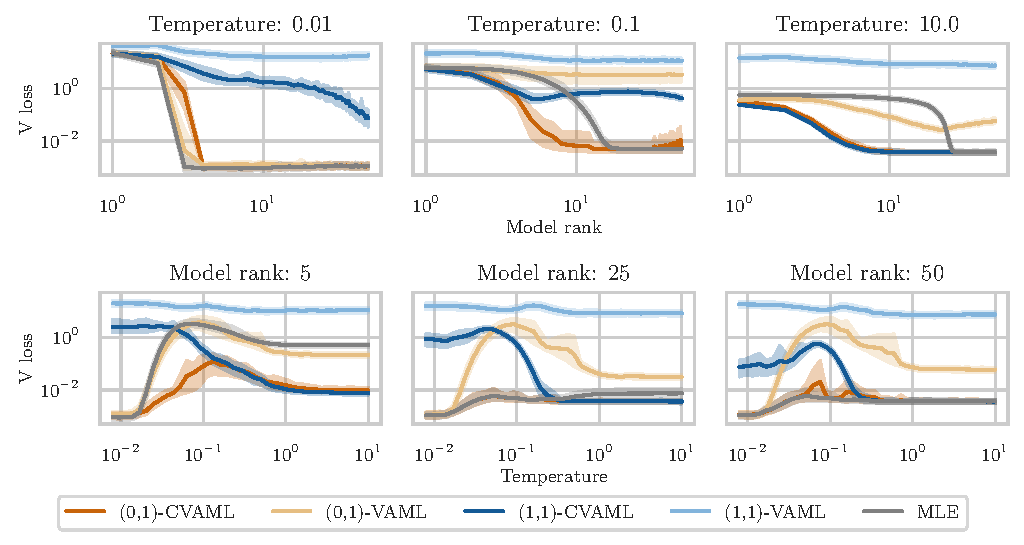
\includegraphics[width=.9\linewidth]{figures/lambda/plts/v_loss_comparison.pdf}
    \caption{Results for the garnet experiments. 
    In the top row, we show the mean squared error of the value function prediction using different latent sizes $k$, over three different temperatures. 
    In the bottom row, we vary the temperature and show results for three values of $k$. 
    Shaded regions are bootstrapped confidence intervals of the mean at 95\% over 1000 independent problems. 
    With the exception of deterministic problems (left), the CVAML loss reliably results in the lowest value prediction error. }
    \label{fig:cvaml:garnet}
\end{figure*}

The problem in the loss function again depends on the variance of the value function with regard to the model.
To overcome this issue, we can introduce another variance correction term, similar to $\hat{\mathcal{L}}_\mathrm{CVAML}$. 
This retains the advantage that the MuZero loss is used for both model and value updates.
However, as we average over the value prediction from the model, we only guarantee that 
\begin{align}
\mathbb{E}_{\hat{p}}\left[V(\hat{x}^{(m)})\right] \approx \mathbb{E}_{\P^\pi}\Bigl[[\mathcal{T}_{\P^\pi}^b V_\mathrm{tar}](x^{m})\Bigr],
\end{align}
not that the values for each state are correct.
These are necessary for accurate planning or policy improvement, therefore, it is still important to use a loss variant with $m=0$ for learning accurate values for each state.

\subsection{Discussion of theoretical results}
While the problem resulting from the use of stochastic models is resolvable, the MuZero loss is still insufficient for learning \emph{per state} value function with stochastic models.
In addition, we observe issues with learning accurate value functions with the $(m\geq1,b\geq1)$-VAML loss even after correctly calibrating it.
If the corrected loss is used to update the model, and a standard model-free or model-based value estimate is used as the value function learning target, the correct value function can be learned.

\begin{boxinsight}[Calibrated losses]
    To obtain a calibrated loss, we propose using $\hat{\mathcal{L}}_\mathrm{CVAML}$ to update the model and $\hat{\mathcal{L}}^{\hat{p}}_{0,j}$, or $\hat{\mathcal{L}}^{\P^\pi}_{0,j}$, to update the value function.
\end{boxinsight}

\section{Calibration impact on finite state MDPs}
\label{sec:cvaml:empirical1}

To test our findings, we run the $(m,b)$-VAML losses on small, finite state Garnet problems \parencite{bhatnagar2007incremental}.
Every problem is generated by sampling $m$ successor states for each state $x_i$, and parameterizing the transitions with random weights $\omega_{i,j}$ for all successor states $x_j$.
The transition distribution is given by $p(x'_i|x_j) = {e^{\omega_{i,j}/\tau}}/{\sum_j e^{\omega_{i,j}/\tau}}$.
Varying the temperature $\tau$ we can interpolate between a deterministic transition and a $m$ uniform one.

The models are parameterized with two learnable matrices $\phi \in \mathbb{R}^{n\times k}$ and $\psi \in \mathbb{R}^{n\times k}$ so that $\hat{p}_k(x_i| x_j)  = \mathrm{softmax}(\hat{\omega}_{i,j}) = \mathrm{softmax}(\phi_i^\top \psi_j)$.
By varying $k$ we create a low-rank constraint.
As \textcite{vaml} shows, $(m,b)$-VAML should be used when the model has insufficient capacity to represent the environment.
As a baseline, we use the model $\hat{p}_{\mathrm{KL}, k}\in \argmin_{\hat{p}} \mathrm{KL}(p\|\hat{p})$.

We focus solely on value estimation in the Garnet MDPs with a fixed policy to simplify the experimental setup.
We also use the ground truth reward function.

\textbf{Results:}
The numerical results are graphed in \autoref{fig:cvaml:garnet}.
For the deterministic ground truth environment, we see no benefit from using a calibrated $(m,b)$-VAML.
We find that the algorithms are able to exploit the non-linear softmax function to achieve very accurate models in deterministic environments.
However, even small amounts of stochasticity prevent this solution.

As the stochasticity increases, we see an advantage for the calibrated losses.
$(1,1)$-VAML is not able to achieve any good results even when the underlying environment is deterministic.
This corroborates the theoretical finding that the error depends on the model's stochasticity and not on the environment.
As we initialize the models with high entropy, $(1,1)$-VAML is unable to learn a high variance value.

Calibrated $(1,1)$-VAML still struggles in environments with low stochasticity.
We find that due to the variance term over value functions, the model is prone to get stuck in local minima as it reduces the value function difference per state faster than the model predictive variance.
This suggests that a $(m\geq1,0)$-CVAML loss is preferable with stochastic environments.

\section{Latent environment models and auxiliary losses}
Prior literature \parencite{lovatto2020decision}, and indeed our own discussion in \autoref{chap:vagram} have found the IterVAML loss to be unstable.
However, we have shown that IterVAML and MuZero are closely related within the $(m,b)$-VAML family, and while the former has been criticized for instability, the later does not have this reputation.
The main difference between prior empirical investigations of IterVAML and MuZero indeed has less to do with the inherent (dis)advantages of the loss functions, and can instead be explained by architectural choices.
In practice, most implementations of MuZero-based models use deterministic latent model structures \parencite{schrittwieser2020mastering,ye2021mastering,hansen2022temporal,antonoglou2022planning}, while IterVAML has mostly been investigated with observation-space models.

This raises two important question: (b) Is the use of \emph{deterministic} models sufficient for modelling transitions for \ac{rl}, especially in the case of stochastic environments, and (b) can the empirical performance differences between different $(m,b)$-VAML losses be understood (mostly) in light of this architectural choice?
We will first address the former question since this can be answered with a formal, mathematical analysis. 

\subsection{Deterministic models for stochastic environments}
\label{sec:cvaml:theory_2}

In general, deterministic function approximations cannot capture the full transition distribution in stochastic environments.
However, it is an open question whether a deterministic \emph{latent} model can be sufficient for learning a value-equivalent model, as conjectured by \textcite{oh2017value}.

We can now answer this question in the affirmative, albeit with some technical caveats: there exist a measurable deterministic model for stochastic environments that perfectly minimizes the $(1,0)$-VAML loss.
Showing the existence of a deterministic value-aware model relies on the continuity of the transition kernel and involved functions $\phi$ and $V$.
These are standard assumptions that are necessary to prove the convergence of many algorithms \parencite{bertsekasshreve1978}. 


The proposition relies on the existence of a deterministic mapping, which we prove here as a lemma.


\begin{lemma}[Deterministic Representation Lemma]
\label{lem:cvaml:deterministic_representation_lemma}
    Let $\mathcal{X}$ be a compact, connected, metrizable space. Let $p$ be a continuous kernel from $\mathcal{X}$ to probability measures over $\mathcal{X}$. Let $\mathcal{Z}$ be a metrizable space. Consider a bijective mapping $\phi: \mathcal{X} \rightarrow \mathcal{Z}$ and any $V: \mathcal{Z} \rightarrow \mathbb{R}$. Assume that they are both continuous. Denote $V_\mathcal{X} = V \circ \phi$.
    
    Then there exists a measurable function $f^*: \mathcal{Z} \rightarrow \mathcal{Z}$ such that we have $V(f^*(\phi(x))) = \EEX{p}{V_\mathcal{X}(x')|x}$ for all $x \in \mathcal{X}$.
\end{lemma}

\begin{proof}
    
Since $\phi$ is a bijective continuous function over a compact space and maps to a Hausdorff space ($\mathcal{Z}$ is metrizable, which implies Hausdorff), it is a homeomorphism.
The image of $\mathcal{X}$ under $\phi$, $\mathcal{Z}_\mathcal{X}$ is then connected and compact.
Since $\mathcal{X}$ is metrizable and compact and $\phi$ is a homeomorphism, $\mathcal{Z}_\mathcal{X}$ is metrizable and compact.
Let $\theta_{V,\mathcal{X}}(x) = \EEX{x' \sim p(\cdot|x)}{V(x')}$.
Then, $\theta_{V,\mathcal{X}}$ is continuous (Proposition \autoref{prop:cvaml:730}).
Define $\theta_{V, \mathcal{X}} = \theta_{V, \mathcal{Z}} \circ \phi$.
Since $\phi$ is a homeomorphism, $\phi^{-1}$ is continuous.
The function $\theta_{V, \mathcal{Z}}$ can be represented as a composition of continuous functions $\theta_{V, \mathcal{Z}} = \theta_{V, \mathcal{X}} \circ \phi^{-1}$ and is therefore continuous.

As $\mathcal{Z}_\mathcal{X}$ is compact, the continuous function $V$ takes a maximum and minimum over the set $\mathcal{Z}_\mathcal{X}$. 
This follows from the compactness of $\mathcal{Z}_\mathcal{X}$ and the extreme value theorem. 
Furthermore $V_{\min} \leq \theta_{V,\mathcal{Z}}(z) \leq V_{\max}$ for every $z \in \mathcal{Z}_\mathcal{X}$.
By the intermediate value theorem over compact, connected spaces, and the continuity of $V$, for every value $V_{\min} \leq v \leq V_{\max}$, there exists a $z \in \mathcal{Z}_\mathcal{X}$ so that $V(z) = v$.


Let $h: \mathcal{Z}_\mathcal{X} \times \mathcal{Z}_\mathcal{X} \rightarrow \mathbb{R}$ be the function $h(z,z') = \abs{\theta_{V,\mathcal{Z}}(z) - V(z')}^2$.
As $h$ is a composition of continuous functions, it is itself continuous.
Let $h^*(z) = \min_{z' \in \mathcal{Z}_\mathcal{X}} h(z,z')$.
For any $z \in \mathcal{Z}_\mathcal{X}$, by the intermediate value argument, there exist $z'$ such that $V(z') = v$. 
Therefore $h^*(z)$ can be minimized perfectly for all $z \in \mathcal{Z}_\mathcal{X}$.

Since $\mathcal{Z}_\mathcal{X}$ is compact, $h$ is defined over a compact subset of $\mathcal{Z}$.
By Proposition \autoref{prop:cvaml:733}, there exists a measurable function $f^*(z)$ so that $\min_{z'} h(z, z') = h(z, f^*(z)) = 0$.
Therefore, the function $f^*$ has the property that $V(f^*(z)) = \EEX{p}{V(z')|z}$, as this minimizes the function $h$.

Now consider any $x\in\mathcal{X}$ and its corresponding $z=\phi(x)$.
As $$h(z, f^*(z))=\abs{\theta_{V,\mathcal{Z}}(z) - V\roundb{f^*(z)}}^2  = 0$$ for any $z \in \mathcal{Z}_\mathcal{X}$, $$V(f^*(\phi(x))) = \theta_{v,\mathcal{Z}}(z) = \EEX{p}{V_\mathcal{X}(x')|x}$$ as desired.

\end{proof}

Equipped with this lemma, we can now prove the main result.

\begin{restatable}{proposition}{DeterministicModel}\label{prop:cvaml:3_1}
    Let $\mathcal{X}$ be a compact, connected, metrizable space. Let $p$ be a continuous kernel from $\mathcal{X}$ to probability measures over $\mathcal{X}$. Let $\mathcal{Z}$ be a metrizable space. Consider a bijective latent mapping $\phi: \mathcal{X} \rightarrow \mathcal{Z}$ and any $V: \mathcal{Z} \rightarrow \mathbb{R}$. Assume that they are both continuous. Denote $V_\mathcal{X} = V \circ \phi$.
    
    Then there exists a measurable function $f^*: \mathcal{Z} \rightarrow \mathcal{Z}$ such that we have $V(f^*(\phi(x))) = \EEX{p}{V_\mathcal{X}(x^{(1)})}$ for all $x \in \mathcal{X}$.

    Furthermore, the same $f^*$ is a minimizer of the expected IterVAML loss:
    $$f^* \in \argmin_{\hat{f}} \EEX{\P^\pi}{\hat{\mathcal{L}}_{\mathrm{IterVAML},1}(\hat{f},V_\mathcal{X}|V_\mathcal{X},x,x^{(1)})}.$$
\end{restatable}

\begin{proof}

As we only deal with single steps here, we use $x^{(1)}$ and $x'$ interchangeably as the latter is simpler and more common nomenclature.
The statement of the proposition itself is written with the $x^{(1)}$ notation to remain consistent with the main body of the paper.

The existence of $f^*$ follows under the stated assumptions (compact, connected, and metrizable state space, metrizable latent space, continuity of all involved functions) from \autoref{lem:cvaml:deterministic_representation_lemma}.

First, expand the equation to obtain:
\begin{align}
     &\EEX{\P^\pi}{\hat{\mathcal{L}}_{\text{IterVAML}, 1}(f, V | V_\mathcal{X} x, x' } \\
    &\quad = \EEX{\P^\pi}{\squareb{V\roundb{f\roundb{\phi(x)}} - V_\mathcal{X}(x')}^2}\\
    &\quad = \EEX{\P^\pi}{\Bigl(V\roundb{f\roundb{\phi(x)}}} - \EEX{\P^\pi}{V_\mathcal{X}(x^{(1)})} + \EEX{\P^\pi}{V_\mathcal{X}(x' - V_\mathcal{X}(x^{(n)}) \Bigr)^2}.
\end{align}
After expanding the square, we obtain three terms:
\begin{align}
    & \EEX{\hat{p},\P^\pi}{\hat{\mathcal{L}}_{\text{IterVAML}, 1}(f, V | V_\mathcal{X} x, x') } \\
    = &\EEX{\hat{p},\P^\pi}{\left|{V\roundb{f\roundb{\phi(x)}} - \EEX{\P^\pi}{V_\mathcal{X}(x')}}\right|^2} \\
    &\quad + 2 \EEX{\P^\pi}{\squareb{V\roundb{f\roundb{\phi(x)}} - \EEX{\P^\pi}{V_\mathcal{X}(x')}}\squareb{\EEX{\P^\pi}{V_\mathcal{X}(x')} - V_\mathcal{X}(x') }}\\
    &\quad + \EEX{\P^\pi}{\left|{\EEX{\P^\pi}{V_\mathcal{X}(x')} - V_\mathcal{X}(x') }\right|^2}
\end{align}

Apply the tower property to the inner term to obtain: 
\begin{align}
&2\EEX{\P^\pi}{\squareb{V\roundb{f\roundb{\phi(x)}} - \EEX{\P^\pi}{V_\mathcal{X}(x')}}\squareb{\EEX{\P^\pi}{V_\mathcal{X}(x')} - V_\mathcal{X}(x') }}\\
&\quad =2\EEX{\P^\pi}{\squareb{V\roundb{f\roundb{\phi(x)}} - \EEX{}{V_\mathcal{X}(x')}}\underbrace{\EEX{\P^\pi}{\EEX{\P^\pi}{V_\mathcal{X}(x')} - V_\mathcal{X}(x') \middle|x'}}_{=0}} = 0.
\end{align}

Since the statement we are proving only applies to the minimum of the IterVAML loss, we will work with the $\argmin$ of the loss function above.
The resulting equation contains a term dependent on $f$ and one independent of $f$:
\begin{align}
    \argmin_f~ & \EEX{\P^\pi}{\left|{V\roundb{f\roundb{\phi(x)}} - \EEX{\P^\pi}{V_\mathcal{X}(x')}}\right|^2} + \EEX{\P^\pi}{\left|{\EEX{\P^\pi}{V_\mathcal{X}(x')} - V_\mathcal{X}(x') }\right|^2}\\
    =~ \argmin_f~ & \EEX{\P^\pi}{\left|{V\roundb{f\roundb{\phi(x)}} - \EEX{\P^\pi}{V_\mathcal{X}(x')}}\right|^2}.
\end{align}

Finally, it is easy to notice that $V\roundb{f^*\roundb{\phi(x)}} = \EEX{\P^\pi}{V_\mathcal{X}(x')}$ by the definition of $f^*$.
Therefore $f^*$ minimizes the final loss term and, due to that, the IterVAML loss.

\end{proof}

We can conclude that given a sufficiently flexible function class $\mathcal{F}$, $(m,b)$-VAML can recover an optimal deterministic model for value function prediction.
Note that our conditions solely ensure the \emph{existence} of a measurable function; the learning problem might still be very challenging.

\subsection{Auxiliary losses}

While the original MuZero algorithm only uses the MuZero loss to update the latent embedding, dynamics model, and value function estimation, several more recent works add auxiliary stabilizing losses \parencite{ye2021mastering,hafner2021mastering,hansen2024tdmpc,voelcker2025mad}.
These allow the model to learn meaningful transitions even before the value function is properly approximated, which helps e.g. in sparse-reward environments.

Most prior works use some form of \ac{byol} \parencite{grill2020bootstrap} loss, which minimizes the difference between the next states encoding $\phi(x^{(m)})$ and the model prediction $f^m(x^{(0)})$.
We saw in the previous chapter that such losses can greatly aid in stabilizing value learning.
In addition, latent-self prediction losses like BYOL show a strong synergy with value function learning.
Therefore it stands to reason that using them in an $(m,b)$-VAML setup can also yield strong benefits.

As a reminder, when the difference between next state embedding and model prediction is measured by the $L_2$ norm, the model loss is
\begin{align}
    & \hat{\mathcal{L}}^{\P^\pi}_{\mathrm{model}, m}\left(\hat{f},
\phi, \hat{V}|x\right) = \underbrace{\hat{\mathcal{L}}^{\P^\pi}_{m,b}\left(\hat{f},\phi, \hat{V}|x\right)}_{m,b\mathrm{-VAML}} + \underbrace{\biggl| \hat{f}^m(\phi(x)) - \bigl[\phi(x^{(m)}) \bigr] \biggr|^2}_\mathrm{auxiliary}.
\end{align}

The introduction of a stabilizing loss poses a challenge for the result in \autoref{prop:cvaml:3_1}.
For example, a pre-trained LLM backbone might be used, which is naturally stochastic due to the sampling strategies used to query it.
Therefore, it is still important to have a calibrated surrogate loss for stochastic models, as many use cases make stochastic models attractive.

For a flexible enough model and embedding function class, the perfect \ac{byol}-based model $f^*_\mathrm{aux}$ would predict $\EEX{\P^\pi}{\phi(x')| x}$.
However, $f^*_\mathrm{aux}$ only coincides with the optimal model under the VAML loss iff
\begin{align}
    \EEX{\P^\pi}{\hat{V}(\phi(x^{(1)}))} = \hat{V}\biggl(\EEX{\P^\pi}{\phi(x^{(1)})}\biggr).
\end{align}
This is the case if and only if the value function is linear in the embedding features $\phi$, which is also referred to as a linear expectation model \parencite{wan2019planning}.
However,  learning an embedding in which the value function is linear can be difficult and may not lead to stable model predictions in complex, high-dimensional environments.

An exception to the use of deterministic models is the architecture proposed by \textcite{antonoglou2022planning}.
However, their model and auxiliary loss rely on a biased straight-through gradient estimation.
This introduces complications for finding the optima of the loss function and model class.

\section{Experimental evaluation}
\label{sec:cvaml:latent_experiments}

% \subsection{$(m,b)$-VAML and auxiliary losses}


To summarize our theoretical results, we can state the following
\begin{itemize}
    \item $(m,b)$-VAML losses are uncalibrated, but we can adapt the losses to calibrate them.
    \item If latent model architectures are used, a perfect, deterministic $(1,0)$-VAML model exists, but might not be easily learnable.
    \item Auxiliary losses can be used to stable learning $(m,b)$-VAML models in practice, but might lead to issues when used with deterministic models and stochastic environments.
\end{itemize}

However, it is unclear how large the impact of all these theoretical results is in realistic environments.
Therefore, we are now faced with several empirical questions, which we will answer with experiments on a subset of DMC environments \parencite{tunyasuvunakool2020dmcontrol} encompassing various tasks within the \textit{humanoid} and \textit{dog} domains.
These two domains are the most challenging in the DMC suite, and the standard comparison for current methods \parencite{voelcker2025mad,nauman2024bigger}.

\begin{enumerate}
    \item Do IterVAML and MuZero perform equivalently when used with the same deterministic latent model architecture?
    \item Do $(m,b)$-VAML algorithms improve when combined with auxiliary losses?
    \item Can we observe the effects of calibration on deterministic environments?
    \item Can we observe the effects of calibration in stochastic environments?
\end{enumerate}

\subsection{Experimental setup}

To conduct our experiments we use a variety of neural network based models.

All experiments are conducted with latent model architectures composed of an encoder, a latent dynamics model, and a value and policy function head.
All networks are simple fully collected feed-forward networks whose architectures are identical to those used in the DMC experiments in \autoref{chap:understanding}.
For hyperparameters and further architectural details, see \autoref{app:cvaml:model_design}.

We compare both stochastic and deterministic latent models.
For the stochastic case, the latent models are multivariate, diagonal Gaussian distributions where mean and variance are parameterized by the latent network \cite{pets,janner2019mbpo,paster2021blast}.
In the deterministic case we simply use a feed-forward network.
 
Model roll-outs are produced by sequentially sampling latent states from the model conditional on the initial state and an action sequence using the reparametrization trick. 
\begin{align}
&\hat{p}(\hat{z}'|z,a)=\hat{\mu}(z,a) + \hat{\sigma}(z,a)\cdot\varepsilon,\; \varepsilon \sim \mathcal{N}(0,I)
%    &\hat{p}^{m+1}(\hat{z}^{(m+1)}|z,a^{(:m)})\nonumber\\
% &\quad=\mathcal{N}\left(\hat{\mu}(\hat{z}^{(m)},a^{(m)}),\hat{\sigma}(\hat{z}^{(m)},a^{(m)})\right)
\end{align}

The auxiliary loss for stochastic models is computed as a negative log-likelihood of the next states' latent representations under the current dynamics model.
\begin{align}
    &\mathcal{L}_{\mathrm{aux},m}\left(\hat{p},\varphi\Big|x,a^{(0:m-1)},x^{(m)}\right) \nonumber\\
    &\quad =-\log \hat{p}^m\left(\varphi(x^{(m)})\Big|\varphi(x),a^{(0:m-1)}\right),
\end{align}
where $a^{(0:m-1)}$ is a sequence of actions of length $m$ starting from state $x^{(0)}$.

In the case of deterministic models, we use the MSE between the next states' representations and the model's predictions:
\begin{align}
    &\mathcal{L}_{\mathrm{aux},m}\left(\hat{p},\varphi\Big|x,a^{(0:m-1)},x^{(m)}\right) \nonumber\\
    &\quad =\left|\left|\hat{p}^m\left(\cdot\Big|\varphi(x),a^{(0:m-1)}\right)-\varphi(x^{(m)}\right|\right|^2
\end{align}

For training the policy and value function, we follow a data-mixing protocol.
We use both model-generated on-policy, and real environment data from the replay buffer to train a value and policy head using the $(m,b)$-VAML loss with a twinned critic parametrization similar to TD3  \cite{fujimoto2018addressing}.
This means the model influences the value function both through the encoder and through on-policy model-generated data.
The impact of the data-mixing strategy will be discussed in further detail in the next chapter, \autoref{chap:mad}.

The actions for environment interactions are obtained from the actor and the environment model using MPC \cite{hansen2022temporal}: initialized at the action produced by the actor for the current state, this algorithm iteratively refines the action to maximize the expected return.
In total our setup uses the model for training the shared encoder, generating data for value and policy improvement, and for online model-based search.

For $(m,b)$-CVAML, the calibration term is computed by sampling multiple trajectories from the model and calculating the means and variances of next-state values produced by the critic across the different samples.

We plot aggregated final performance over 20 random seeds per environment-loss pair with 95\% CI,  estimated with stratified percentile bootstrap \parencite{patterson2024empirical}.
Aggregations of final performance over several environments are visualized using the RLiable library \parencite{agarwal2021deep}.

\subsection{Architecture design and $(m,b)$-VAML stability}
 
We first study the impact of the latent design and auxiliary loss across all tasks.
In \autoref{fig:cvaml:mf_baseline} we compare the $(1,0)$-CVAML (with auxiliary self-prediction loss) with both a model-free TD3 baseline, and with general-purpose models using only the self-prediction loss.
The TD3 baseline is regularized with layer norms to counterbalance the effects described in \autoref{chap:overestimation}.
We found the layer norms recommended by \textcite{hansen2024tdmpc} to be slightly more performant with deep models at low UTD than OFN.

While the dog tasks show small improvements when removing the CVAML loss for deterministic environments, all other models and tasks show a strong drop in performance.
In several cases, using a self-prediction loss even underperforms the model-free baseline.

\label{sec:cvaml:empirical_arch}
\begin{figure}[t]
\centering
    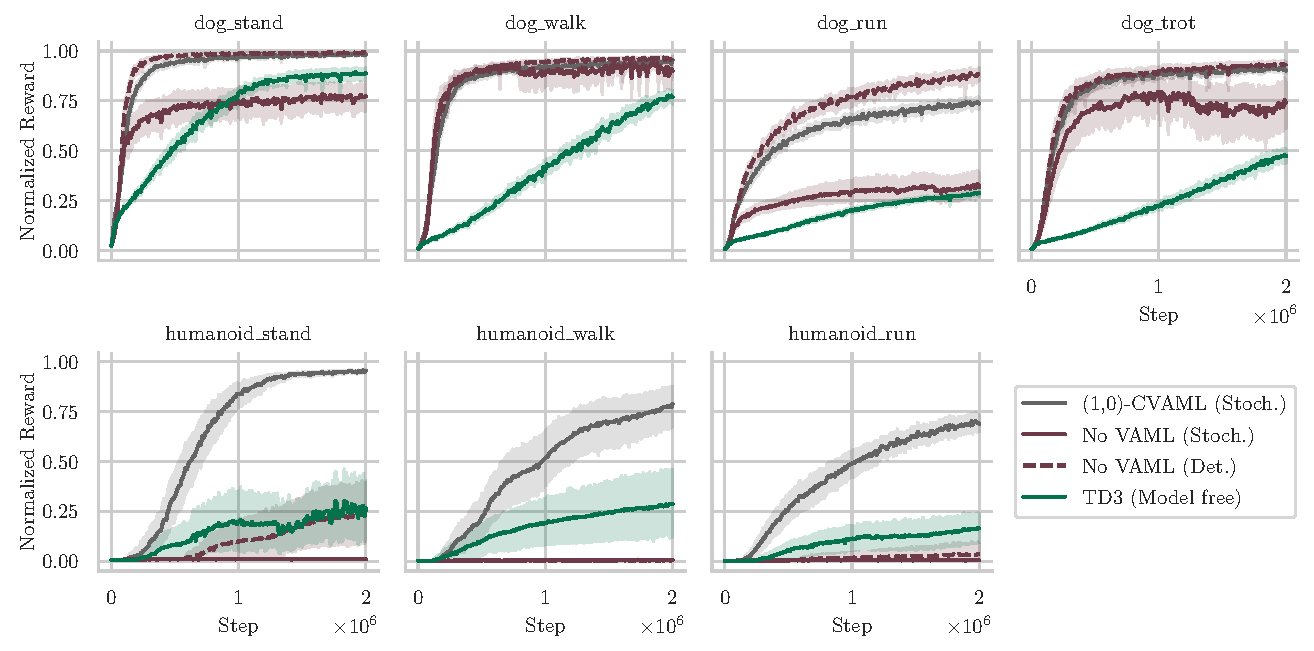
\includegraphics[width=\textwidth]{figures/lambda/plts/ablated_reward1.pdf}
    \caption{Baseline comparison of the CVAML model with a purely general-puprose (only self prediction loss) and model-free baseline. Across all tasks we see a strong performance benefit of the VAML-based model over the model-free and stochastic general-purpose baseline. On some dog tasks, a deterministic self-prediction model performs slightly better than the CVAML variant. However, on the humanoid tasks, performance of the CVAML loss is significantly better than any baseline. In aggregate, CVAML (with an auxiliary task) is a consistenly strong loss.}
    \label{fig:cvaml:mf_baseline}
\end{figure}

In \autoref{fig:cvaml:ablation_itervaml} and \autoref{fig:cvaml:ablation_muzero} we show the results of training $(1,0)$-CVAML and $(1,1)$-CVAML respectively without auxiliary losses.
Comparing the results to the discussion in \autoref{chap:vagram}, we see that the combination of regularized architecture and latent model structure by itself, even without auxiliary self-prediction, leads to stable and performant models.
However, across almost all tasks and model variants, we see increased or identical performance from adding auxiliary latent self-prediction.
The only exception is the humanoid\_ walk task, in which the combined losses perform slightly worse over the course of training.
However, as we will discuss in the next section, this can partially be explained by the lower performance of stochastic architectures on the humanoid tasks.

\begin{figure}[t]
\centering
    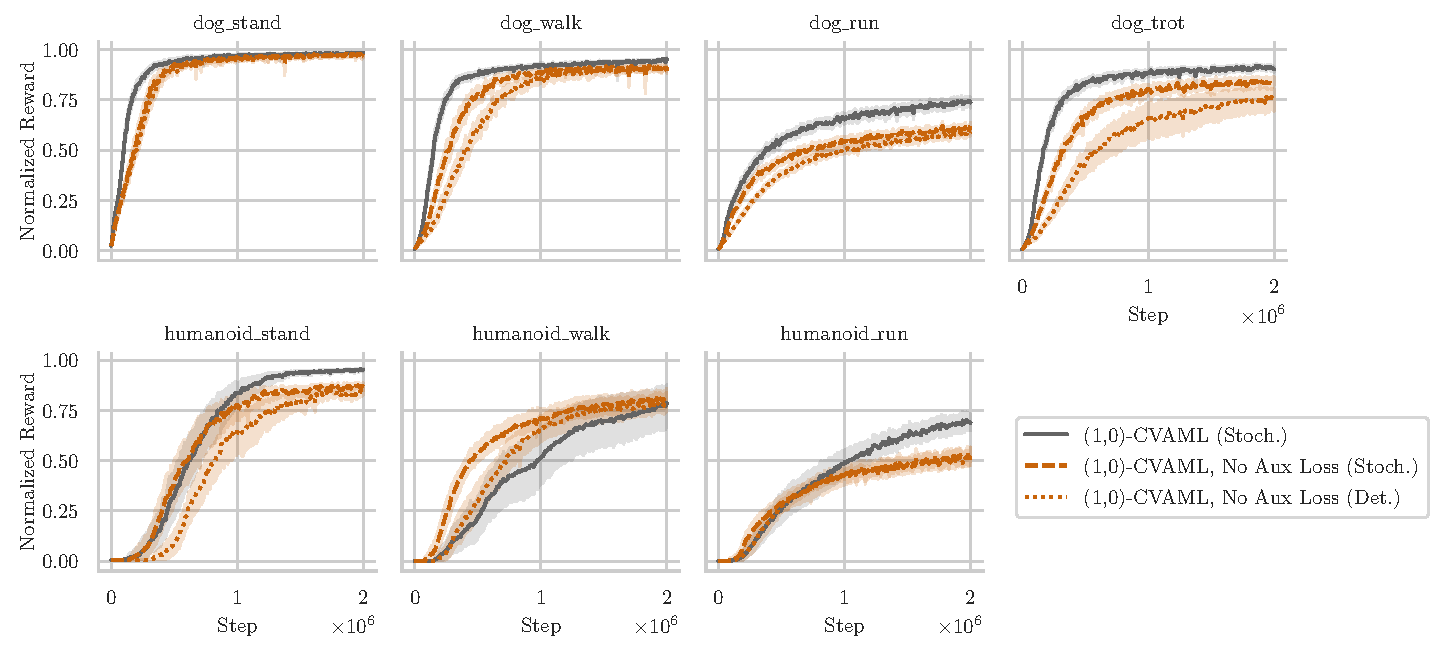
\includegraphics[width=\textwidth]{figures/lambda/plts/ablated_reward2.pdf}
    \caption{Comparison of CVAML with purely decision-aware $(1,0)$-CVAML models (no auxiliary self-prediction loss). With the exception of humanoid\_walk, we see a small but consistent benefit from using an auxiliary loss.}
   \label{fig:cvaml:ablation_itervaml}
\end{figure}


\begin{figure}[t]
\centering
    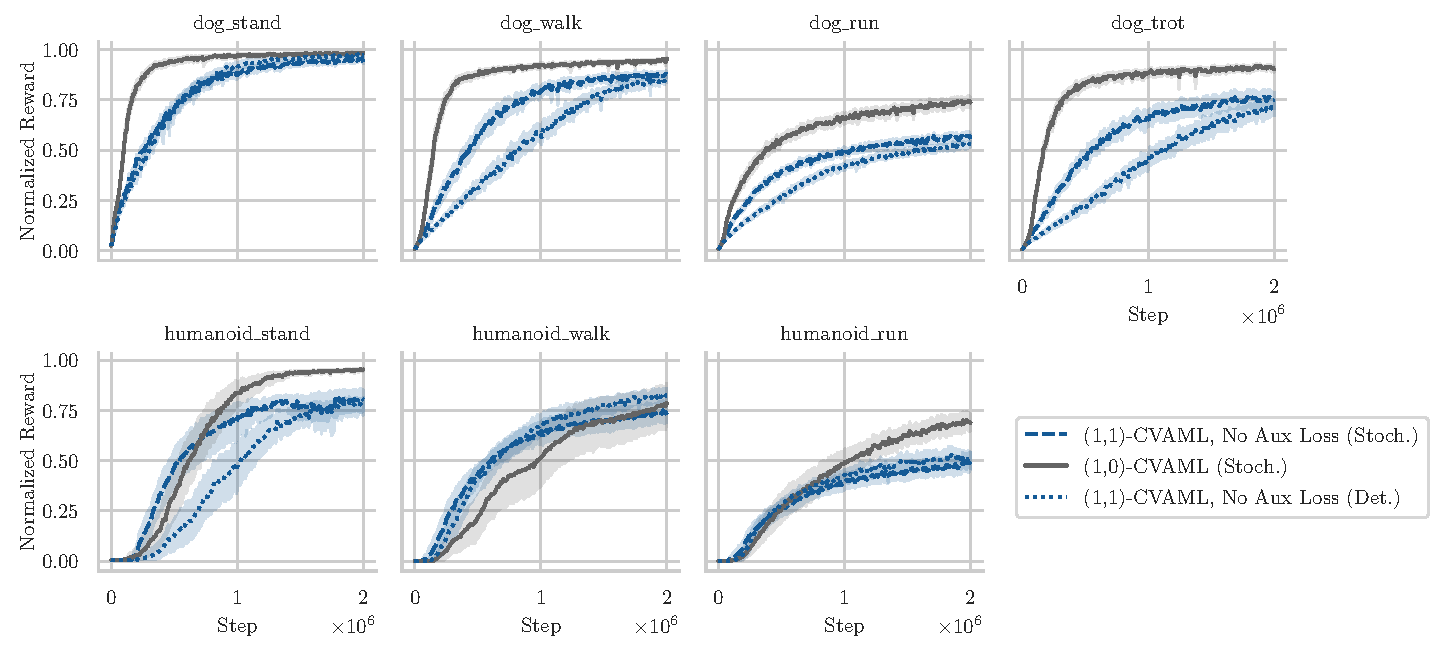
\includegraphics[width=\textwidth]{figures/lambda/plts/ablated_reward3.pdf}
    \caption{Comparison of CVAML with purely decision-aware $(1,1)$-CVAML models (no auxiliary self-prediction loss). With the exception of humanoid\_walk, we see a small but consistent benefit from using an auxiliary loss. In addition, the $(1,0)$ variants outperform the $(1,1)$ variants by a small margin across almost all tasks.}
   \label{fig:cvaml:ablation_muzero}
\end{figure}

\subsection{Calibration experiments with latent-space models}
\label{sec:cvaml:empirical2}

\begin{figure}[t]
\centering
   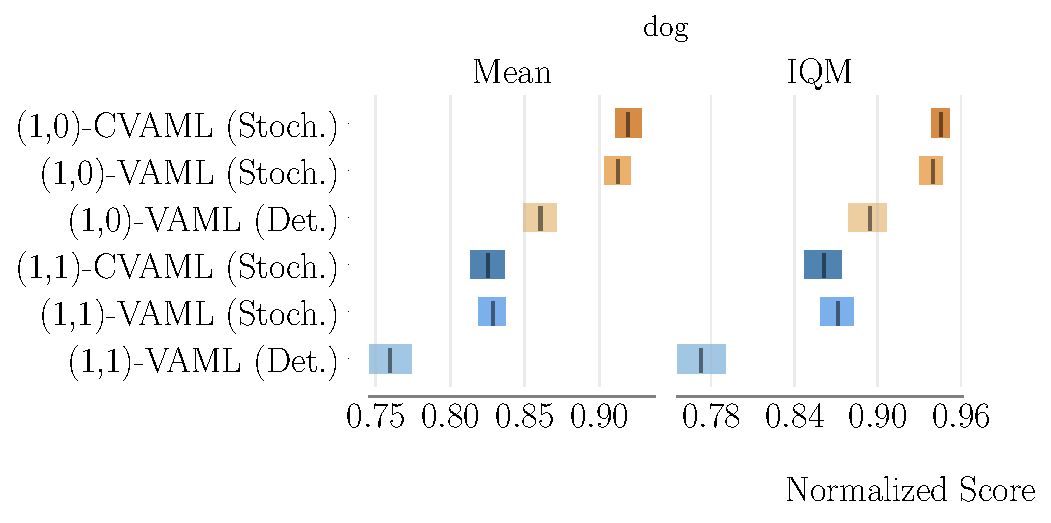
\includegraphics[width=0.5\textwidth]{figures/lambda/plts/agg_dog.pdf} 
   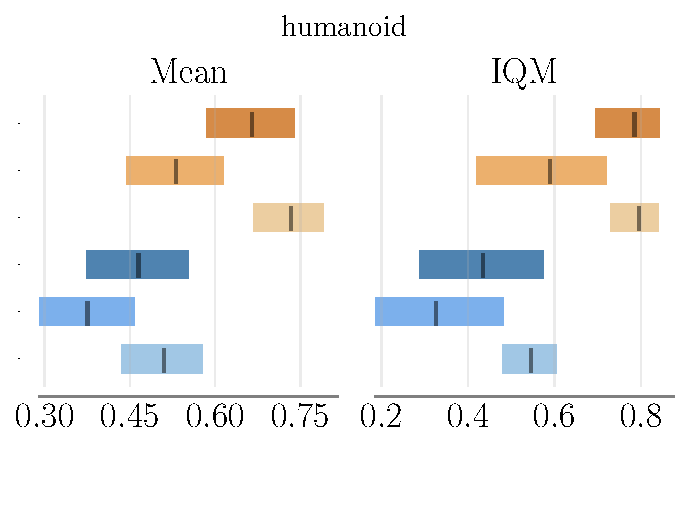
\includegraphics[width=0.33\textwidth]{figures/lambda/plts/agg_hum.pdf} 
   \caption{Results for the latent-space model experiments. We show the aggregate metrics of the final performance on dog (left) and humanoid (right) environments, following \textcite{agarwal2021deep}. Calibrating $(1,1)$-VAML leads to a clear improvement in performance in the dog environment, while for $(1,0)$-(C)VAML the difference is less noticeable. This is consistent with our theoretical findings as learning a smaller variance model can be sufficient, but wrong value functions will be learned with a stochastic model when $b\geq1$.}
   \label{fig:cvaml:agg_results}
\end{figure}

We show aggregated final performance across both DMC domains, dog and humanoid, in \autoref{fig:cvaml:agg_results}.
\autoref{fig:cvaml:dmc_reward} shows aggregated learning curves for each domain.

The difference in performance is most noticeable between the $(1,1)$-VAML and -CVAML, as the uncalibrated loss impacts both model and value function learning in this case. 
This effect is less prominent but still present with $(1,0)$-CVAML, where only the model learning is affected.

In the humanoid domain, we observe a performance improvement when using the calibration with the MuZero-style loss.
In the dog domain, confidence intervals overlap although there is a small trend in the mean.
However, most current algorithms on the dog domain use categorical value representations \parencite{farebrother2024stop}, for which further theoretical analysis is necessary before calibration can be addressed.

In addition to the calibration effect, we observe that probabilistic models outperform deterministic ones in the dog domain, even though the simulator is deterministic.
This is in line with the claims in some prior work \parencite{pets,janner2019mbpo}, as stochastic models can reduce the tendency of the critic to exploit model errors.
However, this advantage seems to be domain-specific and is not replicated in the humanoid suite.

Finally, we observe a consistent advantage of $(0,1)$-updates over the $(1,1)$-updates.
\autoref{fig:cvaml:total_agg} shows that averaged across all environments we obtain a clear gap between all variants of the $(1,0)$-VAML loss over the $(1,1)$-VAML loss. 
In combination with the results from the previous section, we can therefore conclude that $(1,0)$-VAML losses can indeed lead to strong performance.
% A wider empirical investigation into the merits of both IterVAML and MuZero style learning is an important direction for future work.

\begin{boxinsight}[Remarks for practitioners]
While deterministic models are theoretically sufficient for learning value-equivalent models, we observe benefits in some benchmarks from the use of stochastic models.
Using calibrated losses is empirically especially important for MuZero-style model and value updates.
\end{boxinsight}

\begin{figure*}[t]
    \centering
    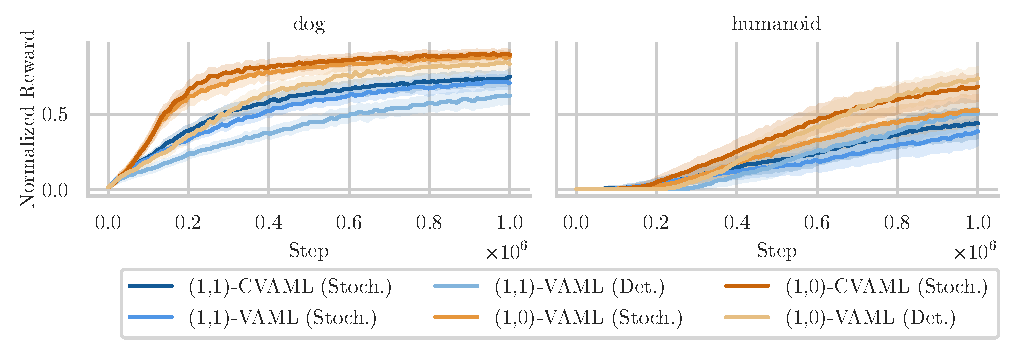
\includegraphics[width=0.8\textwidth]{figures/lambda/plts/reward.pdf} 
    \caption{Sample efficiency curve for both dog (left) and humanoid (right). Per-task normalized return is aggregated over 20 seeds per environment and 3 environments, with 95\% bootstrapped confidence intervals shaded. 
    In addition to a higher final return, we observe significantly earlier learning for the $(0,1)$-(C)VAML on the dog task.}
   \label{fig:cvaml:dmc_reward}
\end{figure*}

\begin{figure*}[b]
    \centering
    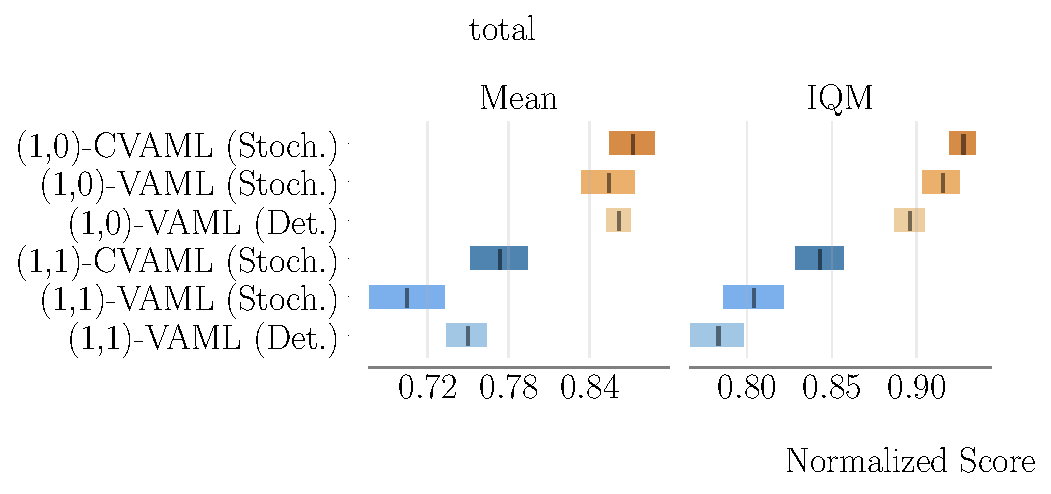
\includegraphics[width=0.5\textwidth]{figures/lambda/plts/agg_total.pdf} 
    \caption{Final performance aggregated across all tasks. We observe that we see a consistent improvement in performance when using $(1,0)$ losses instead of $(1,1)$ losses.}
   \label{fig:cvaml:total_agg}
\end{figure*}

\section{Related work}

\textbf{VAML and MuZero:}~ \textcite{itervaml} established IterVAML based on earlier work \parencite{vaml}.
Several extensions have been proposed, such as a VAML-regularized MSE loss~\parencite{voelcker2022value} and a policy-gradient aware loss \parencite{abachi2020policy}.
Combining IterVAML with latent spaces was first explored by \textcite{abachi2022viper}, but no experimental results were provided.
MuZero \parencite{schrittwieser2020mastering,ye2021mastering} is built based on earlier works which introduce the ideas of learning a latent model jointly with the value function~\parencite{silver2017predictron,oh2017value}.
However, none of these works investigate the calibration of the loss function.
\textcite{antonoglou2022planning} propose an extension to MuZero in stochastic environments but focus on the model architecture, not the value function loss.
\textcite{hansen2022temporal} and \textcite{hansen2024tdmpc} adapted the MuZero loss to continuous control environments but did not extend their formulation to stochastic variants.
\textcite{grimm2020value} and \textcite{grimm2021proper} consider how the set of value equivalent models relates to value functions. 
They are the first to show the close connection between the notions of value-awareness and MuZero.

\textbf{Other decision-aware algorithms:}~ Several other works propose decision-aware model learning algorithms that do not directly minimize a value function difference.
\textcite{doro2020gradient} weigh the samples used for model learning by their impact on the policy gradient.
\textcite{nikishin2021control} uses implicit differentiation to obtain a loss for the model function with regard to the policy performance measure. 
To achieve the same goal, \textcite{eysenbach2022mismatched} and \textcite{ghugare2023simplifying} choose a variational formulation.
\textcite{modhe2021model} proposes to compute the advantage function resulting from different models instead of using the value function.
\textcite{ayoub2020model} presents an algorithm based on selecting models based on their ability to predict value function estimates and provide regret bounds with this algorithm.

\textbf{Learning with suboptimal models:}~ Several works have focused on the broader goal of using models with errors without addressing the loss functions of the model.
Among these, some attempt to correct models using information obtained during exploration~\parencite{joseph2013reinforcement,talvitie2017self,modi2020sample,rakhsha2022operator,rakhsha2024maximum}, or to limit interaction with wrong models~\parencite{buckman2018sample,janner2019mbpo,pmlr-v119-abbas20a}.
Several of these techniques can be applied together with corrected $(m,b)$-VAML to improve the model and value function learning further.
Finally, we do not focus on exploration, but \textcite{guo2022byolexplore} show how auxiliary losses can be used not only to stabilize learning but also to improve exploration.

\section{Conclusions}


We theoretically analyze commonly used value-aware losses such as the MuZero and IterVAML loss and show that they are \emph{uncalibrated} surrogate losses.
When using $(m,b)$-VAML losses, such as the popular IterVAML and MuZero algorithms, with stochastic environment models, the loss learns low variance models, even if those do not recover the correct value function.
Building on our proofs, we propose a novel variant of the loss to stabilize learning with stochastic environments and evaluate its efficacy in practice.

Our experiments further show that the calibration of the $(m,b)$-VAML losses is important for obtaining strong learning with stochastic environment models.
In addition, while previous works showed that IterVAML losses can be unstable in practice \parencite{lovatto2020decision,voelcker2022value}, we find that this can be overcome by adapting the latent model architecture used in \textcite{schrittwieser2020mastering} and the auxiliary losses established by \textcite{li2023efficient,hansen2022temporal}.
When combined with a suitable value learning procedure, IterVAML performs on par or better with MuZero in continuous control tasks.
Finally, while $(m,b)$-VAML losses have mostly been used with deterministic environments, our work enables the community to use stochastic models with a calibrated loss and shows the potential merits of this approach in a number of environments.

In the final chapter, we will take a more detailed look at how combining real and model-generated data stabilizes learning.
